% !TEX program = pdflatex
\documentclass{article}
\usepackage[margin=1in]{geometry}
\usepackage{amsmath,amssymb}
\usepackage{hyperref}
\usepackage{booktabs}
\usepackage{array}
\usepackage{verbatim}

\usepackage{tikz}

\title{SyncTeX Multi-Page Test Document}
\author{tex-kitty Test Suite}
\date{\today}

\hypersetup{
  pdfkeywords={
    pdfcat:anim=engine@10-13@6@1
  }
}





\usetikzlibrary{calc}
\tikzset{>=latex} % for LaTeX arrow head

\colorlet{mylightblue}{blue!10}
\colorlet{mydarkblue}{blue!30!black}
\tikzstyle{arrow}=[->,line width=2,mydarkblue]
\tikzstyle{vector}=[->,line width=2,green!50!black]
\tikzstyle{gas}=[top color=red!30,bottom color=blue!20,shading angle=-45]
\tikzstyle{cold gas}=[blue!20]
\tikzstyle{hot gas}=[red!30]
\tikzstyle{knob}=[line width=2,mydarkblue,fill=blue!20!black!70]
\tikzstyle{arm1}=[very thick,mydarkblue,top color=blue!20!black!25,bottom color=blue!20!black!50]
\tikzstyle{arm2}=[very thick,mydarkblue,top color=blue!20!black!50,bottom color=blue!20!black!60]
\tikzstyle{piston1}=[very thick,mydarkblue,top color=blue!20!black!40,bottom color=blue!20!black!50,middle color=blue!20!black!40,shading angle=90]
\tikzstyle{piston2}=[very thick,mydarkblue,top color=blue!20!black!50,bottom color=blue!20!black!60,middle color=blue!20!black!40,shading angle=0]


% ANGLE
\newcommand{\getangle}[3]{%
    \pgfmathanglebetweenpoints{\pgfpointanchor{#2}{center}}
                              {\pgfpointanchor{#3}{center}}
    \global\let#1\pgfmathresult  
}


% ENGINE
\def\engine#1{
  \def\R{2}    % flywheel
  \def\Ra{1.8} % arm attachment on flywheel
  \def\l{5.0}  % arm length
  \def\w{0.2}  % arm width
  \def\wa{0.3} % piston rod width
  \def\ha{1.5} % piston rod length
  \def\wp{3.8} % piston width
  \def\hp{2.0} % piston height
  \def\wt{1.0} % tube width
  \def\W{4.0}  % wall width
  \def\H{8.4}  % wall height
  \def\T{2.5}  % wall thickness
  \def\cl{1.3} % cooling length
  \def\ct{.25} % cooling thickness
  \def\rb{0.1} % bolt
  \def\d{.4*\R}
  \coordinate (O)   at (0,0);
  \coordinate (R)   at (#1:\Ra);
  \coordinate (Pc)  at (0,{\Ra*sin(#1)-sqrt(\l^2-(\Ra*cos(#1))^2)});
  \coordinate (Ph)  at ({\Ra*cos(#1)+sqrt(\l^2-(\Ra*sin(#1))^2)},0);
  \getangle{\ac}{Pc}{R}
  \getangle{\ah}{Ph}{R}
  
  % GAS
  \fill[gas]
    (\W/2-\wt,-\R-\d-\H) \pipeoutside --++
    (0,-\wt) |-++ (-\H,-\H-\d);
  \fill[cold gas] (Pc) ++ (-\W/2,-\ha-.2*\hp) rectangle (\W/2,-\R-\d-\H-.01);
  \fill[hot gas] (Ph) ++ (\ha+.2*\hp,-\W/2) rectangle (\R+\d+\H+.01,\W/2);
  
  % FLYWHEEL
  \draw[very thick,mydarkblue,top color=blue!20!black!40,bottom color=blue!20!black!50,shading angle=0]
    (O) circle (\R);
  \draw[knob] (O) circle (.25*\R);
  
  % PISTON 1 (COLD)
  \draw[arm1,shading angle=\ac-90]
    (Pc) ++ (\ac-90:\w) arc (\ac-90:\ac-270:\w) --
    ($(R)+(\ac-270:\w)$) arc (\ac+90:\ac-90:\w) -- cycle;
  \draw[piston1]
    (Pc) ++ (180:\wa) arc (180:0:\wa) --++ (0,-\ha) --++
    (\wp/2-\wa,0) --++ (0,-\hp) coordinate[midway] (L) --++
    (-\wp,0) --++ (0,\hp) --++ (\wp/2-\wa,0) -- cycle;
  \draw[knob] (R) circle (\rb);a
  \draw[knob] (Pc) circle (\rb);
  
  % PISTON 2 (HOT)
  \draw[arm2,shading angle=\ah-90]
    (Ph) ++ (\ah-90:\w) arc (\ah-90:\ah-270:\w) --
    ($(R)+(\ah-270:\w)$) arc (\ah+90:\ah-90:\w) -- cycle;
  \draw[piston2]
    (Ph) ++ (270:\wa) arc (270:90:\wa) --++ (\ha,0) --++
    (0,\wp/2-\wa) --++ (\hp,0) --++ (0,-\wp) --++ (-\hp,0) --++ (0,\wp/2-\wa) -- cycle;
  \draw[knob] (R) circle (\rb);
  \draw[knob] (Ph) circle (\rb);
  
  % COOLER
  \foreach \x in {-1,1}{
    \draw[mydarkblue,line width=2,fill=blue!80,xscale=\x]
      (\W/2,-\R-\d-.9*\H) --++ (\ct,0) |-++
      (\cl,\ct) |-++ (-\cl,\ct) |-++
      (\cl,\ct) |-++ (-\cl,\ct) |-++
      (\cl,\ct) |-++ (-\cl,\ct) |-++
      (\cl,\ct) |-++ (-\cl,\ct) |-++
      (\cl,\ct) |-++ (-\cl,\ct) |-++
      (\cl,\ct) coordinate (C\x) |-++ (-\cl,\ct) |-++
      (-\ct,\ct);
    \draw[mydarkblue,line width=1.5,fill=red!80,yscale=\x]
      (\R+\d+.9*\H,\W/2) to[out=90,in=0]++ (-2*\ct,2*\ct) --++
      (-.3*\H,0) coordinate (H\x) to[out=180,in=90]++ (-2*\ct,-2*\ct);
  }
  
  % WALL
  \draw[line width=1.7,mydarkblue,double=blue!20!black!60,double distance=\T,line cap=rect]
    (-\W/2,-\R-\d) |-++ (\W-\wt,-\H)
    \pipeoutside --++ (0,\W-\wt) --++ (-\H,0)
    ( \W/2,-\R-\d) |-++ (\H+\d,-\H) |-++ (-\H,\H+\d);
}


\def\pipeoutside{
            to[out=-90,in=180]++ (\wt,-\wt) --++
  (\H+\d,0) to[out=0,in=-90]++ (\wt,\wt) --++
  (0,\H+\d) to[out=90,in=0]++ (-\wt, \wt)
}

\def\pipeinside{
            to[out=-90,in=180]++ (\wt,-\wt) --++
  (\H+\d,0) to[out=0,in=-90]++ (\wt,\wt) --++
  (0,\H+\d) to[out=90,in=0]++ (-\wt, \wt)
}













\begin{document}
\maketitle
\tableofcontents
\newpage

\section{Purpose}
\label{sec:purpose}
This document is intentionally designed for SyncTeX testing in Neovim with tex-kitty and pdfcat.
Each section contains line-dense content, lists, equations, and references so you can test both
source-to-PDF and PDF-to-source jumps.

Primary checks:
\begin{enumerate}
  \item Cursor on a source line should jump to the right rendered region.
  \item Repeated compilation should keep navigation stable after edits.
  \item Cross-page jumps should still land on the expected logical location.
\end{enumerate}

Reference target for later: Section~\ref{sec:tables}.

\newpage
\section{Paragraph Blocks}
\label{sec:paragraphs}
SyncTeX mappings are easier to verify when paragraphs have unique wording and punctuation.
This paragraph includes short and long lines to create varied line wrapping in the PDF output.
The next paragraph contains deliberate phrase repetition for visual targeting.

The quick brown fox revisits the exact same sentence anchor:
``The quick brown fox jumps over the lazy dog''.
If source jumps are off by one line, this phrase helps detect it quickly.

Another block with mixed punctuation: commas, semicolons; parentheses (including nested markers),
and inline math $a^2+b^2=c^2$.
We also include a hyperlink target: \href{https://www.latex-project.org}{LaTeX Project}.

\newpage
\section{Math Region}
\label{sec:math}
Inline math: $f(x)=\sin(x)+x^2$.
Displayed math:
\begin{equation}
\label{eq:energy}
E = mc^2
\end{equation}

Aligned equations:
\begin{align}
\label{eq:series}
S_n &= \sum_{k=1}^{n} k = \frac{n(n+1)}{2}, \\
T_n &= \sum_{k=1}^{n} k^2 = \frac{n(n+1)(2n+1)}{6}.
\end{align}

Matrix sample:
\[
A =
\begin{bmatrix}
1 & 2 & 3 \\
0 & 1 & 4 \\
0 & 0 & 1
\end{bmatrix}
\]

Cross-reference check: Equation~\ref{eq:energy} and Equation~\ref{eq:series}.

\newpage
\section{Lists and Nested Structure}
\label{sec:lists}
\subsection{Unordered List}
\begin{itemize}
  \item First bullet line for cursor targeting.
  \item Second bullet line with \texttt{monospace} snippet.
  \item Third bullet line with inline math $x \mapsto x+1$.
\end{itemize}

\subsection{Ordered List}
\begin{enumerate}
  \item Step one: compile the file.
  \item Step two: trigger SyncTeX source-to-PDF.
  \item Step three: use PDF-to-source and compare cursor landing.
\end{enumerate}

\subsection{Description List}
\begin{description}
  \item[Input] Source buffer line number.
  \item[Transform] SyncTeX index resolution.
  \item[Output] Page and vertical offset in the PDF viewer.
\end{description}

\newpage
\section{Tables and Alignment}
\label{sec:tables}
\begin{table}[h]
\centering
\begin{tabular}{>{\raggedright\arraybackslash}p{0.3\linewidth}cc}
\toprule
Component & Status & Notes \\
\midrule
Compile hook & pass & Opens viewer only when needed \\
SyncTeX view & pass & Jumps by source line \\
PDF refresh & pass & File watcher driven \\
\bottomrule
\end{tabular}
\caption{High-level integration checkpoints}
\end{table}

Alignment check paragraph: this line is intentionally short.
This next line is intentionally much longer to force wrapping and to provide another
distinct visual anchor for navigation tests.

\newpage
\section{Verbatim and Special Characters}
\label{sec:verbatim}
Special characters in prose: \# \$ \% \& \_ \{ \} \textasciitilde{} \textasciicircum{}.

\begin{verbatim}
for i in range(5):
    print("sync target", i)
\end{verbatim}

Use this region to test whether cursor jumps land exactly around fixed-width blocks,
which often reveal off-by-one behavior in line mapping.

\newpage
\section{Cross References}
\label{sec:refs}
Jump targets:
\begin{itemize}
  \item Return to Purpose section: Section~\ref{sec:purpose}
  \item Go to Math region: Section~\ref{sec:math}
  \item Go to Tables section: Section~\ref{sec:tables}
\end{itemize}

This paragraph exists mainly to provide extra line density on this page.
Make a small edit in this section and recompile to test whether file watcher refresh
keeps the pane stable while preserving smooth navigation behavior.

\newpage
\section{Final Page}
\label{sec:final}
This is the final page used for end-of-document jump validation.
Useful checks:
\begin{enumerate}
  \item Jump from this page back to Section~\ref{sec:purpose}.
  \item Jump to Equation~\ref{eq:energy}.
  \item Confirm that recompiling does not relaunch the viewer process.
\end{enumerate}

End of SyncTeX test document.


\newpage


% 1
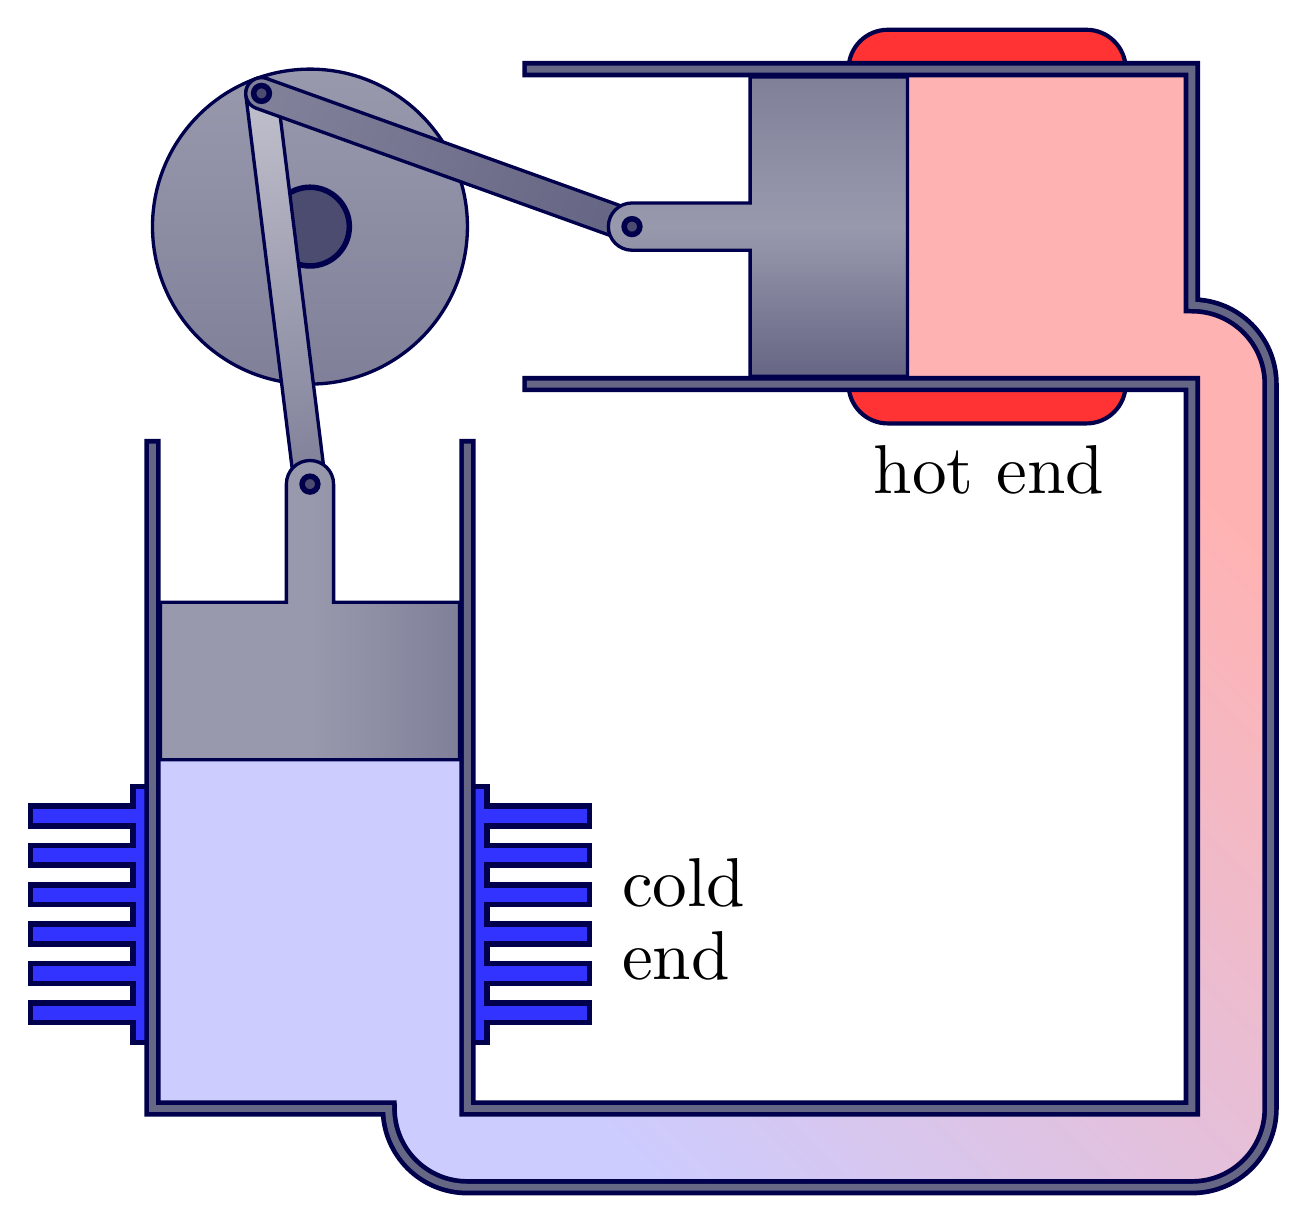
\begin{tikzpicture}
  %\def\d{-10}
  \engine{110};
  %\draw[vector] (\d:.6*\R) arc (\d:\d-80:.55*\R);
  
  \node[below right=3,align=left,scale=2.5] at (C1) {cold\\[-.5mm]end};
  \node[left=13,below right=-1,scale=2.5] at (H-1) {hot end};
%  \node[right=2,align=left,scale=2.5] at (20:1.1*\R) {fly\\[-.5mm]wheel};
%  \draw[arrow] (L) ++ (-.6,-.1) --++ (10:2)
%    node[right=-2,align=right,scale=2.4] {loosely\\[-.5mm]fitting\\[-.5mm]piston};
  
\end{tikzpicture}


% 2
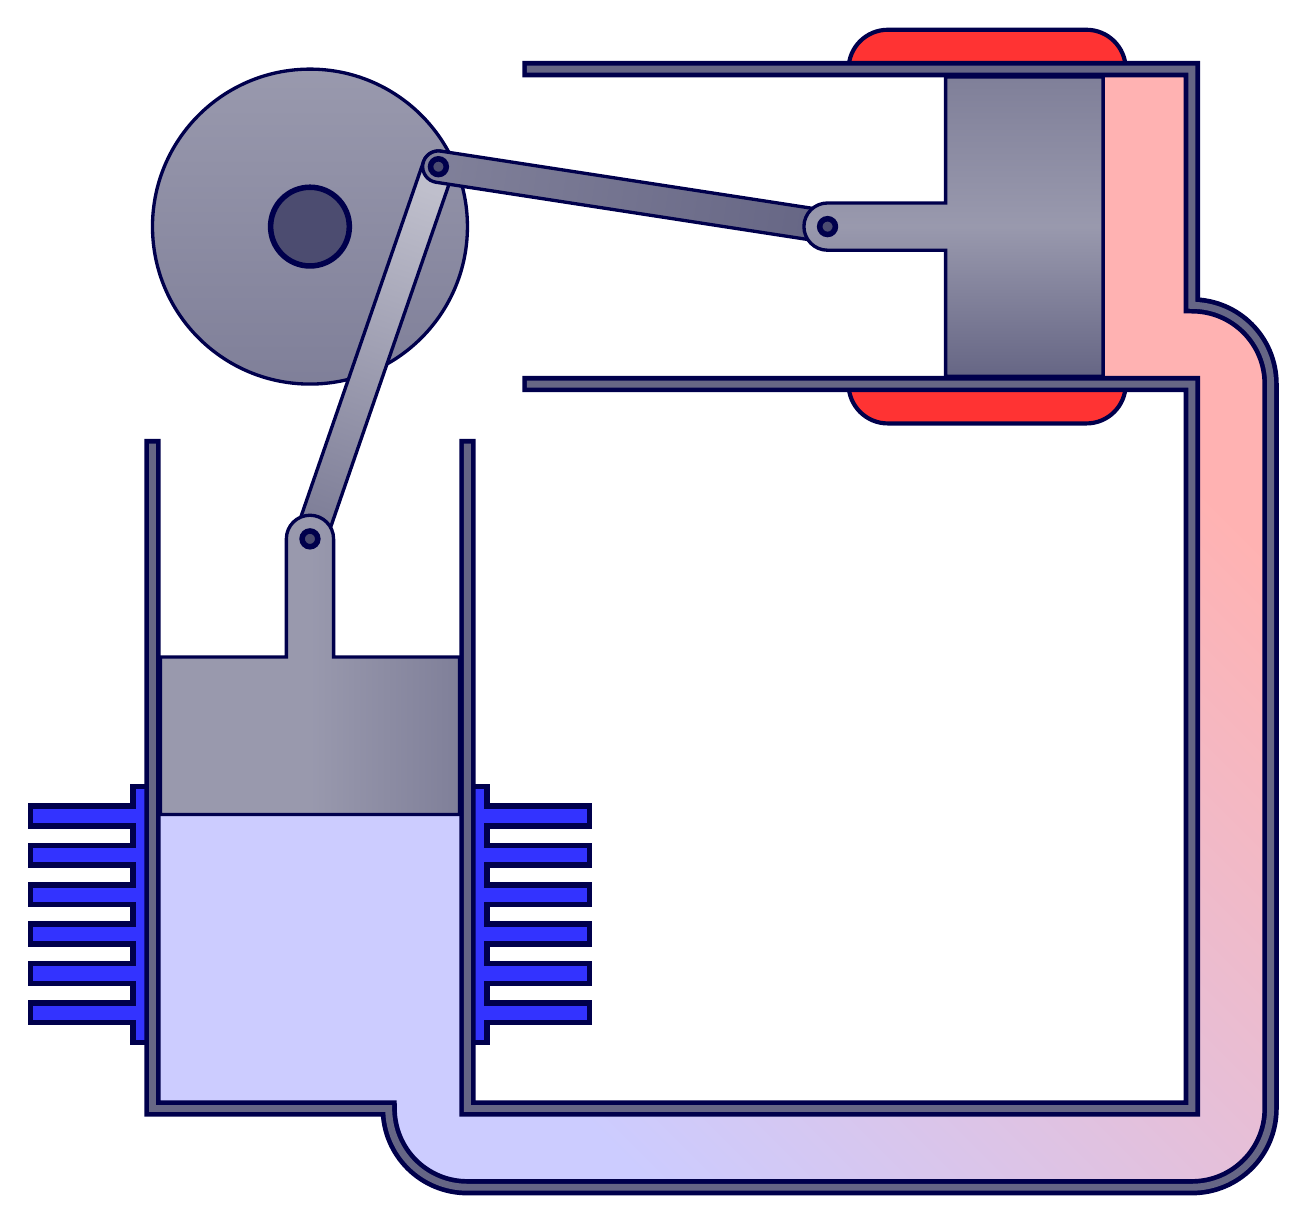
\begin{tikzpicture}
  \engine{25};
\end{tikzpicture}


% 3
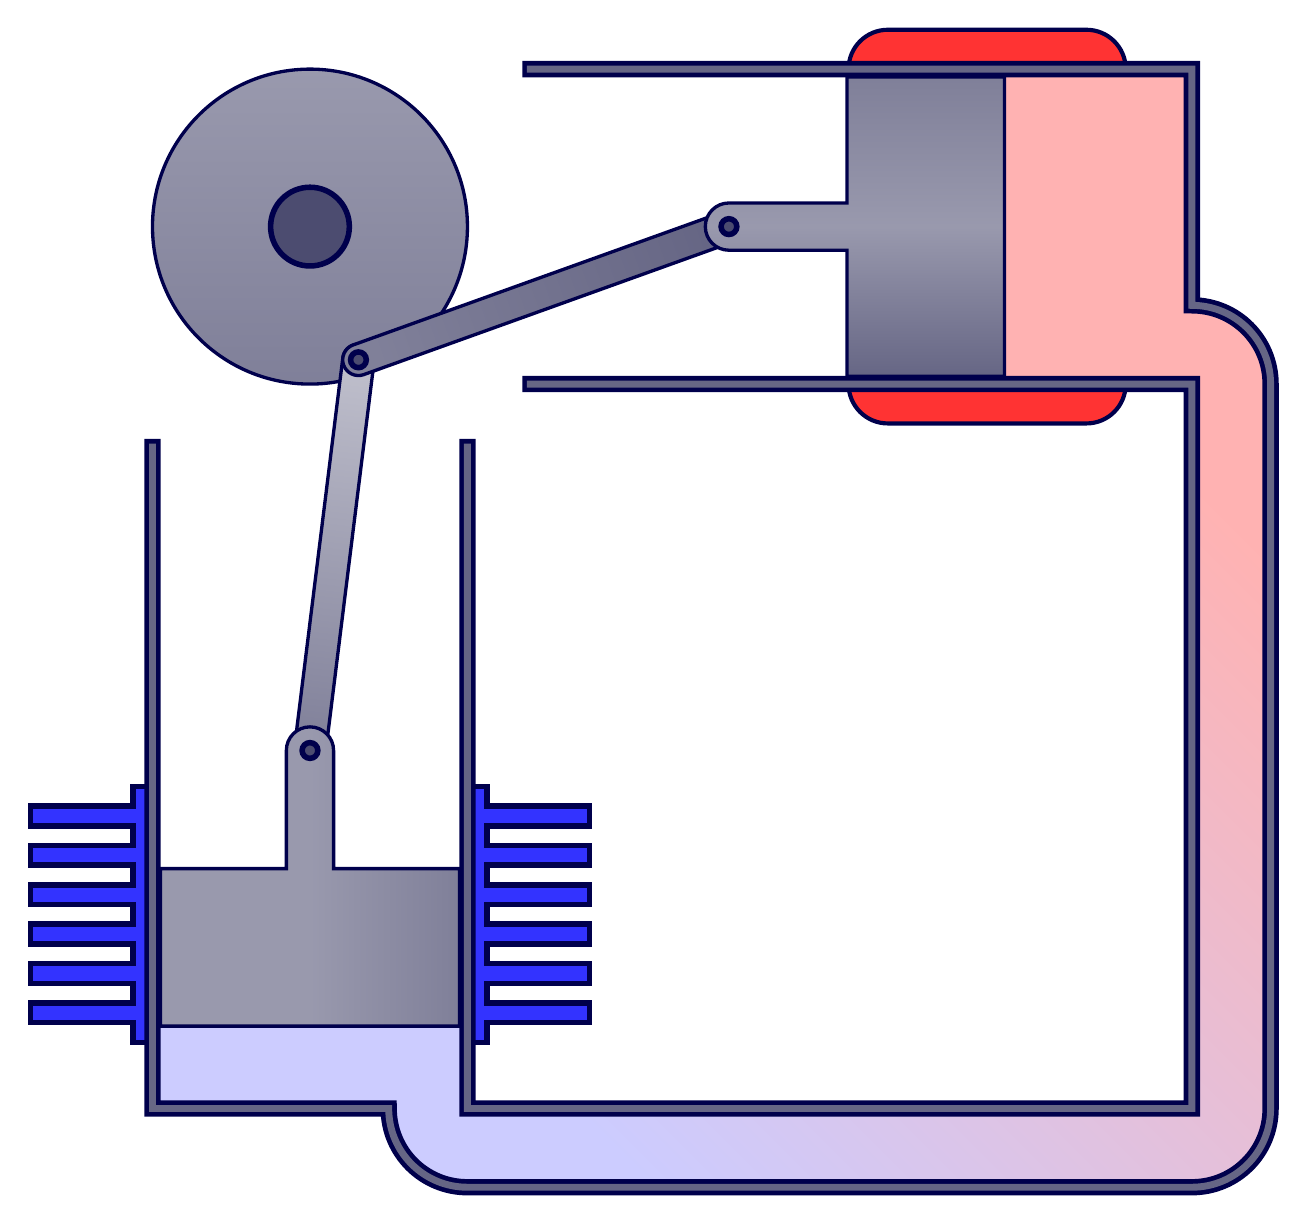
\begin{tikzpicture}
  \engine{-70};
\end{tikzpicture}


% 4
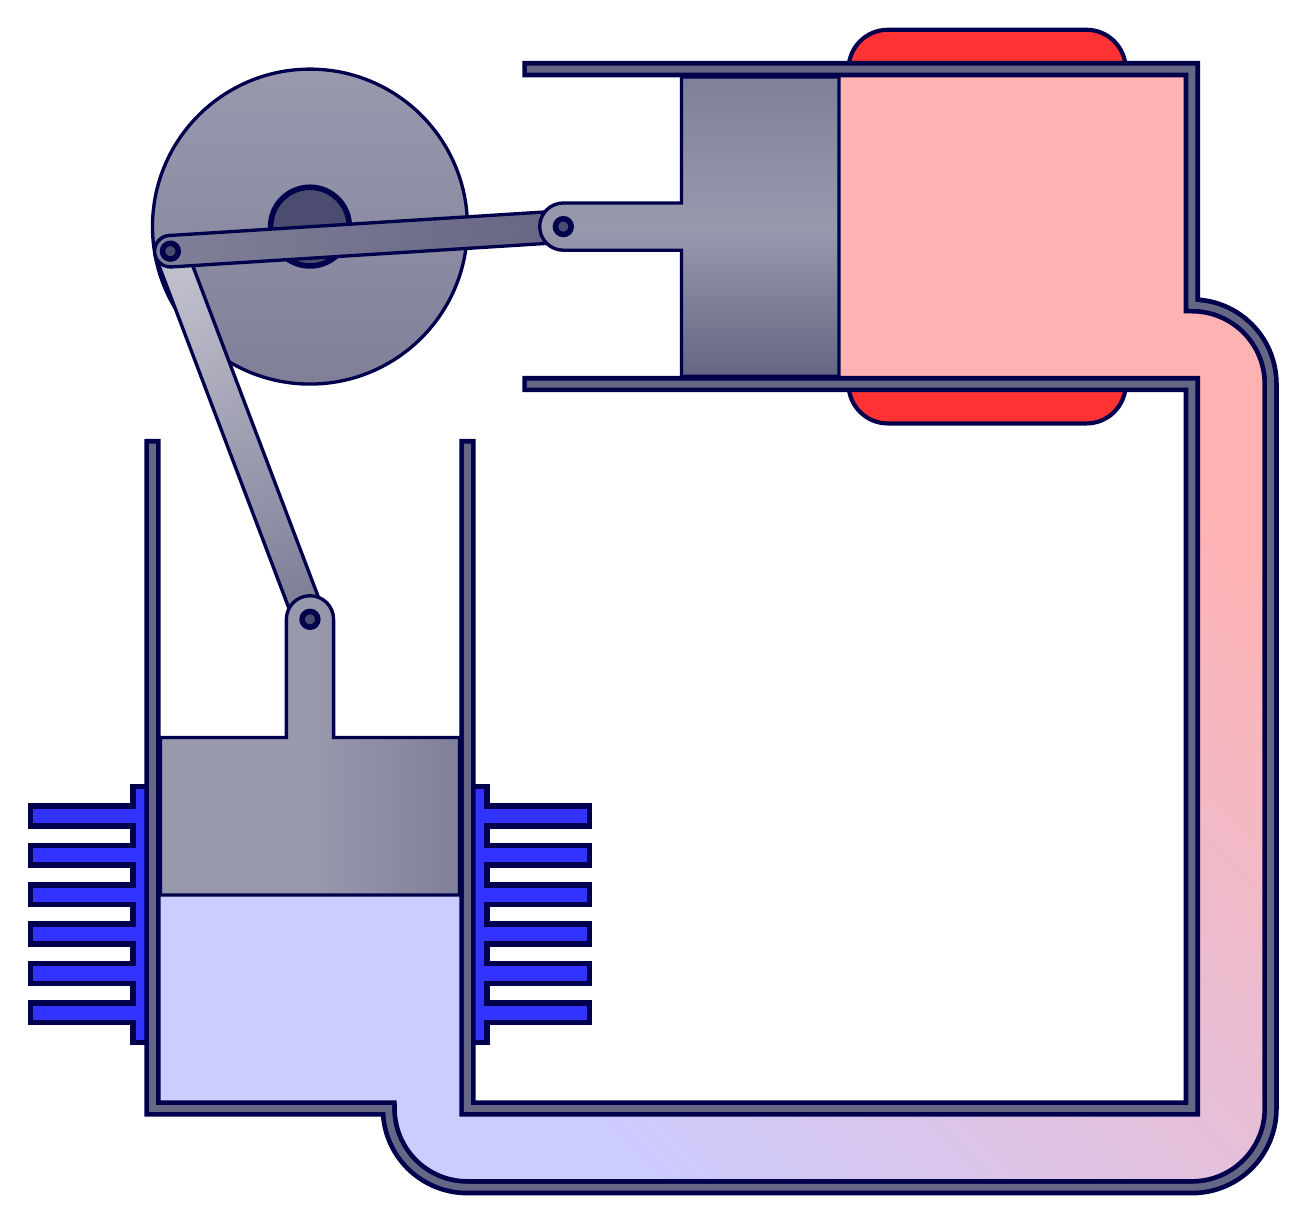
\begin{tikzpicture}
  \engine{-170};
\end{tikzpicture}



\newpage



\section{Some other section}

This proved the loop stops correctly at the end of the file, and that jumps
from the last page back to earlier sections work as expected.



\end{document}
